\chapter{Gocator}
\label{Cha:gocator}
\thispagestyle{empty}

Il Gocator è un sistema di visione 3D che cattura la forma e la posizione di un oggetto, indipendentemente dal colore della superficie e senza opportune calibrazioni.\\
\newline
Il design semplice e flessibile del Gocator consente alle fabbriche di ridurre i costi e massimizzare la redditività migliorando l'efficienza nella convalida dei prodotti. Esso riesce a supportare le richieste di misure 3D accurate, dalle aziende, in settori quali: fusione di alluminio, gomma e produzione di pneumatici, lavorazione del legno, assemblaggio di automobili, food \& packaging, medicale ecc..\\

\begin{figure}[H]
	\centering
	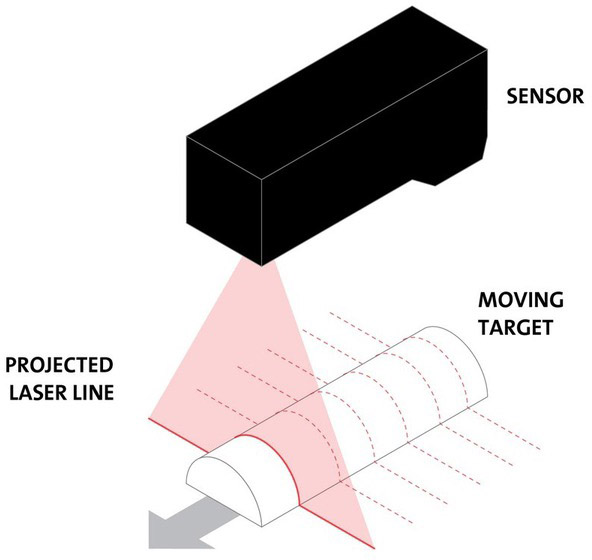
\includegraphics[scale=0.30]{./pictures/gocator_1.jpg}
	\caption{Funzionamento di un profilometro laser.}\label{fig:gocator_1}
\end{figure}

\newpage

\noindent Il modello che è stato utilizzato per l'esecuzione del progetto è il Gocator 2350, facente parte della serie 2300, disponibile in cinque modelli standard, che hanno come caratteristiche comuni:

\begin{itemize}
	\item \textbf{Risoluzione megapixel:} 1280 punti per risoluzione del profilo;
	\item \textbf{Campo visivo:} fino a 1260 mm;
	\item \textbf{Campo di misura:} fino a 800 mm;
\end{itemize}

\ \\
\noindent In particolare, il modello 2350 presenta le seguenti caratteristiche: 

\begin{itemize}
	\item \textbf{Risoluzione dell'asse X:} 0.150 mm;
	\item \textbf{Risoluzione dell'asse Z:} 0.019 mm;
	\item \textbf{Campo visivo (FOV):} 158 mm - 365 mm;
	\item \textbf{Distanza minima (CD):} 300 mm;
	\item \textbf{Campo di misura (MR):} 400 mm;
\end{itemize}

\begin{figure}[H]
	\centering
	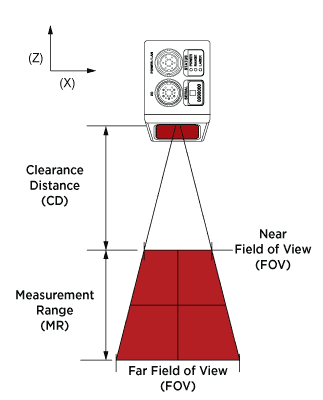
\includegraphics[scale=0.60]{./pictures/gocator_2.png}
	\caption{Caratteristiche visive del Gocator.}\label{fig:gocator_2}
\end{figure}

\section{Settaggi}
Il collegamento tra il sensore e il PC avviene tramite cavo Ethernet, quindi è importante conoscere l'indirizzo IP del Gocator. Una volta identificato l'indirizzo IP, basta inserirlo nel browser web per interagire con l'interfaccia web che LMI mette a disposizione dell'utente.\\
\newline
Per i nostri propositi sono stati modificati alcuni settaggi che rimarranno immutati anche durante le scansioni, mentre i settaggi che potrebbe essere utile modificare in \textit{runtime}, si troveranno anche nella nostra applicazione.

\subsection{Area Attiva}
L'area attiva si riferisce alla regione all'interno del massimo campo visivo del sensore, utilizzata per la profilatura laser (figura \ref{fig:active_area}). Riducendo l'area attiva, il sensore può funzionare a velocità più elevate.\\
\newline
Per i nostri scopi, è stata scelta una dimensione di area attiva di:

\begin{itemize}
	\item \textbf{X Field of View:} 300 mm;
	\item \textbf{Measurement Range:} 250 mm;
\end{itemize}

\begin{figure}[H]
	\centering
	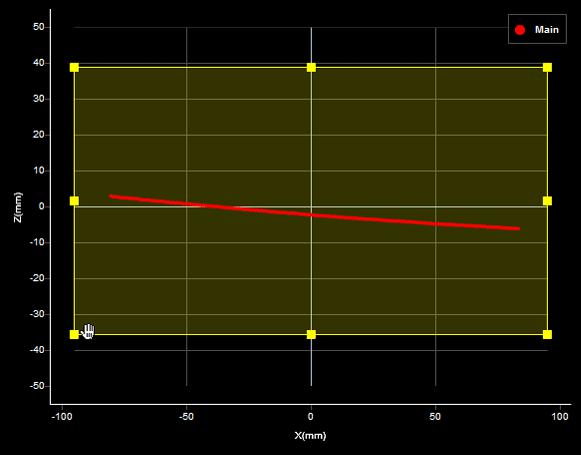
\includegraphics[width=0.7\columnwidth]{./pictures/active_area.png}
	\caption{Il box di colore giallo è l'area attiva. La linea rossa indica l'inclinazione del laser sul conveyor.}\label{fig:active_area}
\end{figure}

\subsection{Trasformazioni}
Le impostazioni di trasformazione determinano come i profili vengono convertiti dalle coordinate del sensore alle coordinate del sistema.\\
\newline
In pratica, i seguenti settaggi servono per allineare il sensore:

\begin{itemize}
	\item \textbf{X Offset:} Specifica lo spostamento lungo l'asse X.
	\item \textbf{Y Offset:} Specifica lo spostamento lungo l'asse Y.
	\item \textbf{Z Offset:} Specifica lo spostamento lungo l'asse Z.
	\item \textbf{Angle X:} Specifica l'inclinazione intorno l'asse X.
	\item \textbf{Angle Y:} Specifica l'inclinazione intorno l'asse Y.
	\item \textbf{Angle Z:} Specifica l'inclinazione intorno l'asse Z.
\end{itemize}

\subsection{Triggers}
Il trigger è un evento che fa sì che il sensore acquisisca una singola immagine.\\

Esso può essere attivato da una delle sorgenti seguenti:

\begin{itemize}
	\item \textbf{Time:} Il sensore ha un clock interno che può essere utilizzato per generare trigger di frequenza fissa.
	\item \textbf{Encoder:} Il trigger viene fornito da un encoder in risposta al movimento.
	\item \textbf{External Input:} Un ingresso digitale può fornire trigger di risposta a eventi esterni.
	\item \textbf{Software} Il trigger è inviato da un comando di rete.
\end{itemize}

\noindent Non avendo a disposizione un encoder, è stata utilizzata la sorgente \textit{time} con il massimo \textit{frame rate} disponibile (183.413 Hz) che è stato sincronizzato con la velocità del conveyor.

\subsection{Esposizione}
L'esposizione determina la durata del tempo della fotocamera e del laser. Esposizioni più lunghe possono essere utili per rilevare i segnali laser su superfici scure o distanti, ma aumentando il tempo di esposizione si riduce la velocità massima.\\
\newline
Il Gocator fornisce tre modalità di esposizione per scansionare diversi tipi di superfici: \textit{Single}, \textit{Dynamic}, \textit{Multiple}.\\
Per i battistrada è stata utilizzata l'esposizione singola con un valore di 2000 $\mu$s, perchè la superficie è uniforme ed è la stessa per tutte le parti.\\
\newline
Inoltre, la corretta regolazione dell'esposizione dipende dalle proprietà riflettenti del materiale in esame, per questo è stato scelto di rendere questo parametro editabile direttamente nel nostro programma.

\subsection{Filtri}
Il software di LMI permette di utilizzare dei filtri per post-elaborare i dati di scansione, in modo da pulirli e rimuovere il rumore.\\
La scelta è ricaduta nel disattivarli tutti per avere delle \textit{point cloud} quanto più "pulite" possibili.

\newpage

\section{Metodi di scansione}
Il Gocator supporta i seguenti metodi di scansione:

\begin{itemize}
	\item Acquisizione superficie;
	\item Acquisizione intensità;
\end{itemize}

\subsection{Acquisizione superficie}
Con questo metodo, il sensore genera una superficie (\textit{point cloud}) combinando una serie di profili raccolti lungo il conveyor.\\
\newline
La generazione delle \textit{point cloud} può avvenire applicando diverse modalità:

\begin{itemize}
	\item \textbf{Continuous:} il sensore genera superfici solo quando vengono rilevate;
	\item \textbf{Fixed length:} il sensore genera superfici di lunghezza fissa (in mm) utilizzando un valore settato da noi;
	\item \textbf{Variable length:} il sensore genera superfici di lunghezza variabile;
	\item \textbf{Rotational:} usata per eseguire scansioni di oggetti circolari;
\end{itemize}

\noindent Per i nostri scopi, è stata scelta la modalità \textbf{continuous}.\\
\newline
Per quanto riguarda la generazione dei dati delle \textit{point cloud}, il Gocator permette di produrle in due formati:

\begin{itemize}
	\item Con dati \textbf{grezzi} (non elaborati);
	\item Con \textbf{spaziatura uniforme} (ricampionati);
\end{itemize}

\subsubsection{Spaziatura uniforme}
Con questo formato, gli intervalli vengono ricampionati con una spaziatura uniforme lungo l'asse \textit{X}, che quindi viene divisa in "contenitori" di dimensioni fisse.\\
\newline
I punti del profilo che cadono nello stesso "contenitore", vengono combinati in un unico valore (\textit{Z}).\\
\newline
Un intervallo più ampio crea profili con una risoluzione \textit{X} inferiore, riduce l'utilizzo della CPU e potenzialmente aumenta la frequenza dei fotogrammi. Di contro, riduce la velocità di output dei dati.\\

\begin{figure}[H]
	\centering
	\begin{subfigure}{.3\linewidth}
		\centering
		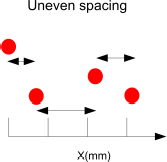
\includegraphics[width = \linewidth]{./pictures/uniform_spacing_1.png}
    	\caption{Con dati grezzi}
    \end{subfigure}
    \hspace{1em}
    \begin{subfigure}{.3\linewidth}
		\centering
		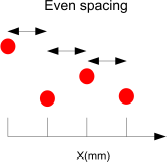
\includegraphics[width = \linewidth]{./pictures/uniform_spacing_2.png}
    	\caption{Con spaziatura uniforme}
    \end{subfigure}
    \caption{Confronto con e senza spaziatura uniforme.}
    \label{fig:uniform_spacing}
\end{figure}

\subsection{Acquisizione intensità}
Con questo metodo, verrà prodotto un valore di intensità (0-255) per ciascun punto scansionato dal laser. In pratica viene misurata la quantità di luce riflessa dall'oggetto.

\subsection{Metodo scelto}
Per i nostri scopi, ovviamente, è stato scelto il metodo dell'acquisizione della superficie con una spaziatura uniforme di 0.15 mm.